
%%%%%%%%%%%%%%%%

% designed to be integrated with conceptual figure

%%%%%%%%%%%
\documentclass[border=0.2cm,12pt]{standalone}
 
\usepackage{tikz}
\usetikzlibrary{positioning,automata}
\usetikzlibrary{arrows,backgrounds,calc,trees}
\usetikzlibrary{hobby} % last answer from https://tex.stackexchange.com/questions/70999/highlight-a-group-of-nodes-in-a-tikz-tree

\tikzset{>=latex} % for LaTeX arrow head
\usepackage{xcolor}

% taken from neural networks
\usepackage{amsmath} % for aligned
%\usepackage{amssymb} % for \mathbb
%\usepackage{etoolbox} % for \ifthen
\usepackage{listofitems} % for \readlist to create arrays
\usetikzlibrary{arrows.meta} % for arrow size
\usepackage[outline]{contour} % glow around text
\contourlength{1.4pt}

\newcommand{\F}{\mathcal{F}}

% to draw hulls between groups of nodes
% taken from 
% https://tex.stackexchange.com/questions/70999/highlight-a-group-of-nodes-in-a-tikz-tree
\pgfdeclarelayer{background}
\pgfsetlayers{background,main}
\newcommand{\convexpath}[2]{
[   
    create hullnodes/.code={
        \global\edef\namelist{#1}
        \foreach [count=\counter] \nodename in \namelist {
            \global\edef\numberofnodes{\counter}
            \node at (\nodename) [draw=none,name=hullnode\counter] {};
        }
        \node at (hullnode\numberofnodes) [name=hullnode0,draw=none] {};
        \pgfmathtruncatemacro\lastnumber{\numberofnodes+1}
        \node at (hullnode1) [name=hullnode\lastnumber,draw=none] {};
    },
    create hullnodes
]
($(hullnode1)!#2!-90:(hullnode0)$)
\foreach [
    evaluate=\currentnode as \previousnode using \currentnode-1,
    evaluate=\currentnode as \nextnode using \currentnode+1
    ] \currentnode in {1,...,\numberofnodes} {
  let
    \p1 = ($(hullnode\currentnode)!#2!-90:(hullnode\previousnode)$),
    \p2 = ($(hullnode\currentnode)!#2!90:(hullnode\nextnode)$),
    \p3 = ($(\p1) - (hullnode\currentnode)$),
    \n1 = {atan2(\y3,\x3)},
    \p4 = ($(\p2) - (hullnode\currentnode)$),
    \n2 = {atan2(\y4,\x4)},
    \n{delta} = {-Mod(\n1-\n2,360)}
  in 
    {-- (\p1) arc[start angle=\n1, delta angle=\n{delta}, radius=#2] -- (\p2)}
}
-- cycle
}

% using tableau 10 color palette: https://public.tableau.com/views/TableauColors/ColorPaletteswithRGBValues?%3Aembed=y&%3AshowVizHome=no&%3Adisplay_count=y&%3Adisplay_static_image=y

\definecolor{myblue}{RGB}{31,119,180}
\definecolor{myred}{RGB}{214,39,40}
\definecolor{mygreen}{RGB}{44,160,44}

% original colors defined by original author
\colorlet{myorange}{orange!70!red!60!black}
\colorlet{mydarkred}{red!30!black}
\colorlet{mydarkblue}{blue!40!black}
\colorlet{mydarkgreen}{green!30!black}
\tikzstyle{node}=[ultra thick,circle,minimum size=30,inner sep=2.,outer sep=0.6]
\tikzstyle{node green}=[node,fill=mygreen]
\tikzstyle{node blue}=[node,fill=myblue]
\tikzstyle{node orange}=[node,orange!20!black,draw=myorange!30!black,fill=myorange!20]
\tikzstyle{node red}=[node,fill=myred]
\tikzstyle{connect}=[thick,mydarkblue] %,line cap=round
\tikzstyle{connect arrow}=[-{Latex[length=4,width=3.5]},thick,mydarkblue,shorten <=0.5,shorten >=1]
\tikzset{ % node styles, numbered for easy mapping with \nstyle
  node 1/.style={node in},
  node 2/.style={node hidden},
  node 3/.style={node out},
}
\def\nstyle{int(\lay<\Nnodlen?min(2,\lay):3)} % map layer number onto 1, 2, or 3
 

% spacing nodes
% \tikzset{node distance = 0.5cm and 0.5cm}

\begin{document}

 
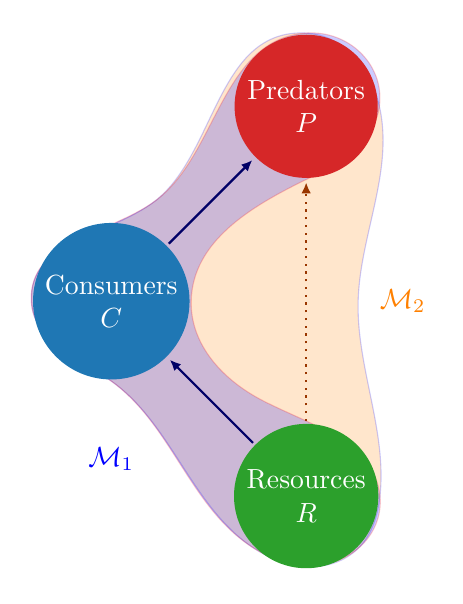
\begin{tikzpicture}[
    node distance=3.5cm,
    on grid,
    very thick,]
 
% Plants
\node [ node green, align=center, text=white] (R) { Resources \\$R$ };
 
% Mode 2    
\node [node blue, align=center, text=white] (C) [above left=of R] { Consumers \\$C$ };
\node (M1) [below= 2cm of C,text=blue]{$\mathcal{M}_1$};
\node (M2) [right=3.7cm of C,text=orange]{$\mathcal{M}_2$};

% Mode 3    
\node [node red, align=center, text=white] (P) [above right=of C]
{ Predators \\ $P$ };


\begin{scope} [connect arrow]  % now dashed is for the lines inside the scope
    \draw (R) -- (C)  ; 
    \draw (C) -- (P)  ; 
    \draw [dotted,myorange] (R) -- node[right]{} (P)  ; 
\end{scope}

% adding the background
\begin{pgfonlayer}{background}
    \draw[blue,fill=orange,opacity=0.2](P.north) to[closed,curve through={($(P.south west)!0.5!(C.north west)$) .. (C.west) .. (C.south) .. (R.south west) .. (R.south east) .. (R.east) .. ($(R.north east)!0.5!(P.south east)$) .. (P.east)}](P.north);

    \draw[red,fill=blue,opacity=0.2](P.north) to[closed,curve through={($(P.south west)!0.5!(C.north west)$) .. (C.west) .. (C.south) .. (R.south west) .. (R.south east) .. (R.east) .. ($(R.north east)!0.5!(C.south east)$) .. (C.east).. (P.south) .. (P.east)}](P.north);
\end{pgfonlayer}



\end{tikzpicture}
 
\end{document}